\section{二重积分}
\subsection{二重积分的概念}
设\(f(x,y)\)是有界闭区域\(D\)上的有界函数.将闭区域\(D\)任意分成\(n\)个小闭区域\[
	\increment\sigma_1,\increment\sigma_2,\dotsc,\increment\sigma_n,
\]
其中\(\increment\sigma_i\)表示第\(i\)个小闭区域,
也表示它的面积.
在每个\(\increment\sigma_i\)上任取一点\(\opair{\xi_i,\eta_i}\),
作乘积\(f(\xi_i,\eta_i) \increment\sigma_i\ (i=1,2,\dotsc,n)\),
并作和\(\sum_{i=1}^n f(\xi_i,\eta_i) \increment\sigma_i\).
如果当各小闭区域的直径中的最大值\(\lambda\)趋于零时,
这和的极限总存在,
则称此极限为
“函数\(f(x,y)\)在闭区域\(D\)上的\DefineConcept{二重积分}(double integral)”,
记作\(\iint_D f(x,y) \dd{\sigma}\),即
\[
	\iint_D f(x,y) \dd{\sigma}
	= \lim_{\lambda\to0}
	\sum_{i=1}^n f(\xi_i,\eta_i) \increment\sigma_i,
\]
其中\(f(x,y)\)叫做\DefineConcept{被积函数},
\(f(x,y) \dd{\sigma}\)叫做\DefineConcept{被积表达式},
\(\dd{\sigma}\)叫做\DefineConcept{面积元素},
\(x\)与\(y\)叫做\DefineConcept{积分变量},
\(D\)叫做\DefineConcept{积分区域},
\(\sum_{i=1}^n f(\xi_i,\eta_i) \increment\sigma_i\)叫做\DefineConcept{积分和}.

如果函数\(f(x,y)\)在闭区域\(D\)上的二重积分存在,
那么就说\(f(x,y)\)在\(D\)上\DefineConcept{可积},
记作\(f \in R(D)\).

在二重积分的定义中对闭区域\(D\)的划分是任意的.
如果在直角坐标系中用平行于坐标轴的直线网来划分\(D\),
那么面积元素\(\dd{\sigma}\)可以改为记作\(\dd{x}\dd{y}\),
进而把二重积分记作\[
	\iint_{D}{f(x,y)\dd{x}\dd{y}},
\]
其中\(\dd{x}\dd{y}\)叫做\DefineConcept{直角坐标系中的面积元素}.

\begin{theorem}[充分条件]
设函数\(f(x,y)\)在闭区域\(D\)上连续,则\(f(x,y)\)在\(D\)上可积.
\end{theorem}

\subsection{二重积分的几何性质}
一般的,如果\(f(x,y) \geq 0\),
被积函数\(f(x,y)\)可解释为曲顶柱体的顶在点\((x,y)\)处的竖坐标,
所以二重积分的几何意义就是柱体的体积.如果\(f(x,y) < 0\),
柱体就在\(xOy\)面的下方,
二重积分的绝对值仍等于柱体的体积,
但二重积分的值是负的.如果\(f(x,y)\)在\(D\)的部分区域上是正的,
而在其他的部分区域上是负的,
那么\(f(x,y)\)在\(D\)上的二重积分就等于
\(xOy\)面上方的柱体体积减去\(xOy\)面下方的柱体体积所得之差.

\subsection{二重积分的性质}
\begin{property}\label{theorem:重积分.二重积分的性质1}
设\(\alpha\)、\(\beta\)为常数,则\[
\iint_D [\alpha f(x,y)+\beta g(x,y)] \dd{\sigma}
=\alpha \iint_D f(x,y) \dd{\sigma}
+\beta \iint_D g(x,y) \dd{\sigma}.
\]
\end{property}

\begin{property}\label{theorem:重积分.二重积分的性质2}
如果闭区域\(D\)被有限条曲线分为有限个部分闭区域,
则在\(D\)上的二重积分等于在各部分闭区域上二重积分的和,
即\[
	D = \bigcup_{i=1}^n D_i
	\implies
	\iint_D f(x,y) \dd{\sigma}
	= \sum_{i=1}^n \iint_{D_i} f(x,y) \dd{\sigma}.
\]
\end{property}
这个性质表示二重积分对于积分区域具有\DefineConcept{可加性}.

\begin{property}\label{theorem:重积分.二重积分的性质3}
如果在\(D\)上,\(f(x,y)=1\),\(\sigma\)为\(D\)的面积,
则\[
	\iint_D 1\cdot\dd{\sigma}
	=\iint_D \dd{\sigma}
	=\sigma.
\]
\end{property}

\begin{property}\label{theorem:重积分.二重积分的性质4}
如果在\(D\)上,\(f(x,y) \leq \phi(x,y)\),
则有\[
	\iint_D f(x,y) \dd{\sigma} \leq \iint_D \phi(x,y) \dd{\sigma}.
\]

特别地,\[
	\abs{\iint_D f(x,y) \dd{\sigma}} \leq \iint_D \abs{f(x,y)} \dd{\sigma}.
\]
\end{property}

\begin{property}\label{theorem:重积分.二重积分的性质5}
设\(M\)、\(m\)分别是\(f(x,y)\)在闭区域\(D\)上的最大值和最小值,
\(\sigma\)是\(D\)的面积,
则有\[
	m\sigma \leq \iint_D f(x,y) \dd{\sigma} \leq M\sigma.
\]
\end{property}
上述不等式对于二重积分估值的不等式.

\begin{property}[二重积分的中值定理]\label{theorem:重积分.二重积分的中值定理}
设函数\(f(x,y)\)在闭区域\(D\)上连续,
\(\sigma\)是\(D\)的面积,
则在\(D\)上至少存在一点\((\xi,\eta)\),
使得\[
	\iint_D f(x,y) \dd{\sigma} = \sigma \cdot f(\xi,\eta).
\]
\begin{proof}
显然\(\sigma\neq0\).
把\cref{theorem:重积分.二重积分的性质5} 中的不等式各除以\(\sigma\),
有\[
	m
	\leq
	\zeta = \frac{1}{\sigma} \iint_D f(x,y) \dd{\sigma}
	\leq
	M.
\]
这就是说,确定的数值\(\zeta\)是
介于函数\(f(x,y)\)的最大值\(M\)与最小值\(m\)之间的.
根据\cref{theorem:多元函数微分法.介值定理},
在\(D\)上存在一点\((\xi,\eta)\)
使得函数在该点的值\(f(\xi,\eta)\)
与上述的确定的数值\(\zeta\)相等,
即\[
	f(\xi,\eta) = \zeta,
\]
上式两端各乘以\(\sigma\),记得所要证明的公式.
\end{proof}
\end{property}

\begin{example}
设\(f(x,y) = f_1(x) \cdot f_2(y)\),证明:\[
	\iint_D f(x,y) \dd{x} \dd{y}
	= \left[ \int_a^b f_1(x) \dd{x} \right] \cdot \left[ \int_c^d f_2(y) \dd{y} \right],
\]
其中\(D = \Set{(x,y) \given a \leq x \leq b, c \leq y \leq d}\).
%TODO proof
\end{example}

\subsection{二重积分的计算法}
直接按照二重积分的定义来计算二重积分,
对少数特别简单的被积函数和积分区域来说是可行的.
但对一般的函数和区域来说,这不是一种切实可行的方法.
这里介绍一种计算二重积分的方法,即把二重积分化为两次单积分(即两次定积分)来计算.

\subsubsection{利用直角坐标系计算二重积分}
如\cref{figure:二重积分.X型区域},
设积分区域\(D\)可以用不等式
\[
	a \leq x \leq b, \qquad
	\phi_1(x) \leq y \leq \phi_2(x)
\]来表示,
其中函数\(\phi_1(x),\phi_2(x)\)在区间\([a,b]\)上连续,
那么有\[
	\iint_D f(x,y) \dd{\sigma}
	= \int_a^b \left[ \int_{\phi_1(x)}^{\phi_2(x)} f(x,y) \dd{y} \right] \dd{x}.
\]

上式右端的积分叫做“先对\(y\)、后对\(x\)的二次积分”.
就是说,先把\(x\)看做常数,把\(f(x,y)\)只看做\(y\)的函数,
并对\(y\)计算从\(\phi_1(x)\)到\(\phi_2(x)\)的定积分;
然后把算得的结果(是\(x\)的函数)对\(x\)计算在区间\([a,b]\)上的定积分.
这个先对\(y\)、后对\(x\)的二次积分也常记作\[
	\int_a^b \dd{x} \int_{\phi_1(x)}^{\phi_2(x)} f(x,y) \dd{y}.
\]
因此也有\[
	\iint_D f(x,y) \dd{\sigma}
	= \int_a^b \dd{x} \int_{\phi_1(x)}^{\phi_2(x)} f(x,y) \dd{y}.
\]
这就是把二重积分化为先对\(y\)、后对\(x\)的二次积分的公式.

\begin{figure}[ht]
	\centering
	\begin{tikzpicture}
		\begin{axis}[
			xmin=1,xmax=3.1,
			axis lines=middle,
			ticks=none,
			enlarge x limits=0.05,
			enlarge y limits=0.5,
			xlabel=$x$,
			ylabel=$y$,
		]
			\coordinate(A)at(1,{sin(2 r)+2});
			\coordinate(B)at(3,{sin(6 r)+2});
			\draw[dashed,black!30](A)--(1,0)node[below,black]{\(a\)}
				(B)--(3,0)node[below,black]{\(b\)};
			\addplot[color=blue,samples=100,smooth,domain=1:3]{sin(\x r)+3};
			\addplot[color=blue,samples=100,smooth,domain=1:3]{sin(2*\x r)+2};
			\draw[blue](A)--(1,{sin(1 r)+3})
				(B)--(3,{sin(3 r)+3});
			\draw(2,{(sin(1 r)+sin(2 r)+sin(3 r)+sin(6 r))*.25+2.5})node{\(D\)};
		\end{axis}
	\end{tikzpicture}
	\caption{}
	\label{figure:二重积分.X型区域}
\end{figure}

类似地,设积分区域\(D\)可以用不等式\[
	\psi_1(y) \leq x \leq \psi_2(y), \qquad
	c \leq y \leq d
\]来表示,
其中函数\(\psi_1(y),\psi_2(y)\)在区间\([c,d]\)上连续,
那么就有\[
	\iint_D f(x,y) \dd{\sigma}
	= \int_c^d \left[ \int_{\psi_1(y)}^{\psi_2(y)} f(x,y) \dd{x} \right] \dd{y}.
\]
上式右端的积分叫做“先对\(x\)、后对\(y\)的二次积分”,
这个积分也常记作\[
	\int_c^d \dd{y} \int_{\psi_1(y)}^{\psi_2(y)} f(x,y) \dd{x}.
\]
因此又有\[
	\iint_D f(x,y) \dd{\sigma}
	= \int_c^d \dd{y} \int_{\psi_1(y)}^{\psi_2(y)} f(x,y) \dd{x}.
\]
这就是把二重积分化为先对\(x\)、后对\(y\)的二次积分的公式.

X型区域\(D\)的特点是:
任一穿过\(D\)内部且平行于\(y\)轴的直线与\(D\)的边界相交不多于两点.
Y型区域\(D\)的特点是:
任一穿过\(D\)内部且平行于\(x\)轴的直线与\(D\)的边界相交不多于两点.

如果积分区域\(D\)既是X型的,可用不等式\[
	a \leq x \leq b, \qquad
	\phi_1(x) \leq y \leq \phi_2(x)
\]表示,
又是Y型的,可用不等式\[
	\psi_1(y) \leq x \leq \psi_2(y), \qquad
	c \leq y \leq d
\]表示,
则有\[
	\int_a^b \dd{x}
	\int_{\phi_1(x)}^{\phi_2(x)} f(x,y) \dd{y}
	=\int_c^d \dd{y}
	\int_{\psi_1(y)}^{\psi_2(y)} f(x,y) \dd{x}.
\]
上式表明,这两个不同次序的二次积分相等,因为它们都等于同一个二重积分\[
	\iint_D f(x,y) \dd{\sigma}.
\]

但是,在化二重积分为二次积分时,为了计算简便,需要选择恰当的二次积分的顺序.
这时,既要考虑积分区域\(D\)的形状,又要考虑被积函数\(f(x,y)\)的特性.

\subsubsection{利用极坐标计算二重积分}
有些二重积分,积分区域\(D\)的边界曲线用极坐标方程来表示比较方便,
且被积函数用极坐标变量\(\rho\)、\(\theta\)表达比较简单.
这时,就可以考虑利用极坐标来计算二重积分.

下面我们按二重积分的定义\[
	\iint_D f(x,y) \dd{\sigma}
	= \lim_{\lambda\to0} \sum_{i=1}^n f(\xi_i,\eta_i) \increment\sigma_i
\]来研究一下这个和的极限在极坐标系中的形式.

\begin{figure}[ht]
	\centering
	\begin{tikzpicture}
		\begin{polaraxis}[
			ticks=none,
			enlarge y limits=0.05,
			axis x line=none,
			axis y line=middle,
			xmin=0,xmax=90,
			xlabel=A,
		]
			\addplot[color=blue,samples=100,smooth,domain=20:40]{sin(3*x)};
			\draw[dashed,black!30](20,{sin(60)})coordinate(A)
				--(0,0)node[above right,black]{\(O\)}coordinate(O)
				--(40,{sin(120)})coordinate(B);
			\addplot[color=blue,samples=100,smooth,domain=20:40]{1.1-.5*sin(3*x)};
			\draw[blue](A)--(20,{1.1-.5*sin(60)})coordinate(C)
				(B)--(40,{1.1-.5*sin(120)})coordinate(D);
			\draw(30,{.75*sin(90)})node{\(D\)};
			\coordinate(P)at(0,1);
			\draw pic["$\alpha$",draw=orange,->,angle eccentricity=1.5,angle radius=5mm]{angle=P--O--A};
			\draw pic["$\beta$",draw=orange,->,angle eccentricity=1.3,angle radius=10mm]{angle=P--O--B};
		\end{polaraxis}
	\end{tikzpicture}
\end{figure}

假定从极点\(O\)出发且穿过闭区域\(D\)内部的射线与\(D\)的边界曲线相交不多于两点.
我们用以极点为中心的一族同心圆\(\rho = \text{常数}\),
以及从极点出发的一族射线\(\theta = \text{常数}\),
把\(D\)划分为\(n\)个小闭区域.
除了包含边界点的一些小闭区域外,其他小闭区域的面积\(\increment\sigma_i\)可计算如下:
\begin{align*}
	\increment\sigma_i
	&= \frac{1}{2} (\rho_i+\increment\rho_i)^2 \cdot \increment\theta_i
	- \frac{1}{2} \rho_i^2 \cdot \increment\theta_i \\
	&= \frac{1}{2} (2\rho_i + \increment\rho_i) \increment\rho_i \cdot \increment\theta_i \\
	&= \frac{\rho_i + (\rho_i+\increment\rho_i)}{2}
		\cdot \increment\rho_i \cdot \increment\theta_i \\
	&= \overline{\rho}_i \cdot \increment\rho_i \cdot \increment\theta_i,
\end{align*}
其中\(\overline{\rho}_i\)表示相邻两端圆弧的半径的平均值.
在这小闭区域内取圆周\(\rho = \overline{\rho}_i\)上的
一点\(\opair{\overline{\rho}_i,\overline{\theta}_i}\),
该点的直角坐标设为\(\opair{\xi_i,\eta_i}\),
则由直角坐标系与极坐标系之间的关系有\(\xi_i = \overline{\rho}_i \cos\overline{\theta}_i,
\eta_i = \overline{\rho}_i \sin\overline{\theta}_i\).
于是\[
	\lim_{\lambda\to0} \sum_{i=1}^n f(\xi_i,\eta_i) \increment\sigma_i
	= \lim_{\lambda\to0} \sum_{i=1}^n
	f(\overline{\rho}_i \cos\overline{\theta}_i,\overline{\rho}_i \sin\overline{\theta}_i)
	\overline{\rho}_i \cdot \increment\rho_i \cdot \increment\theta_i,
\]
即\[
	\iint_D f(x,y) \dd{\sigma}
	= \iint_D f(\rho\cos\theta,\rho\sin\theta) \rho \dd{\rho} \dd{\theta}.
\]

这里我们把点\((\rho,\theta)\)看作在同一平面上的点\((x,y)\)的极坐标表示,
所以上式右端的积分区域仍然记作\(D\).

由于在直角坐标系中\(\iint_D f(x,y) \dd{\sigma}\)也常记作\(\iint_D f(x,y) \dd{x} \dd{y}\),
所以上式又可以写成
\begin{equation}\label{equation:线性方程组.二重积分坐标变换公式}
\iint_D f(x,y) \dd{x} \dd{y}
= \iint_D f(\rho\cos\theta,\rho\sin\theta) \rho \dd{\rho} \dd{\theta},
\end{equation}
这就是二重积分的变量从直角坐标变换为极坐标的变换公式,
其中\(\rho \dd{\rho} \dd{\theta}\)就是极坐标系中的面积元素.

\cref{equation:线性方程组.二重积分坐标变换公式} 表明,
要把二重积分中的变量从直角坐标变换为极坐标,
只要把被积函数中的\(x\)、\(y\)分别换成\(\rho \cos\theta\)、\(\rho \sin\theta\),
并把直角坐标系中的面积元素\(\dd{x} \dd{y}\)换成极坐标系中的面积元素\(\rho \dd{\rho} \dd{\theta}\).

极坐标系中的二重积分,同样可以化为二次积分来计算.
\begin{theorem}
设积分区域可以用不等式\begin{gather*}
0 \leq \phi_1(\theta) \leq \rho \leq \phi_2(\theta), \\
0 \leq \alpha \leq \theta \leq \beta \leq 2\pi,
\end{gather*}来表示,其中函数\(\phi_1(\theta)\)、\(\phi_2(\theta)\)在区间\([\alpha,\beta]\)上连续,那么利用以下关系\[
\left\{ \begin{array}{l}
x = \rho\cos\theta \\
y = \rho\sin\theta \\
\end{array} \right.
\quad\text{或}\quad
\left\{ \begin{array}{l}
\rho = \sqrt{x^2+y^2} \\
\tan\theta = y/x \quad (x \neq 0) \\
\end{array} \right.,
\]替换二重积分\(\iint_{D}{f(x,y)\dd{x}\dd{y}}\)中的积分变量,即有
\begin{equation}
\iint_D f(\rho\cos\theta,\rho\sin\theta) \rho \dd{\rho} \dd{\theta}
=\int_\alpha^\beta \left[
	\int_{\phi_1(\theta)}^{\phi_2(\theta)}
		f(\rho\cos\theta,\rho\sin\theta) \rho \dd{\rho} \right] \dd{\theta}.
\end{equation}
上式也可写作
\begin{equation}
\iint_D f(\rho\cos\theta,\rho\sin\theta) \rho \dd{\rho} \dd{\theta}
=\int_\alpha^\beta \dd{\theta}
	\int_{\phi_1(\theta)}^{\phi_2(\theta)}
		f(\rho\cos\theta,\rho\sin\theta) \rho \dd{\rho}.
\end{equation}
\end{theorem}

\begin{corollary}
设区域\(D\)在极坐标系中是由射线\(\theta=\alpha\)、\(\theta=\beta\)和曲线\(\rho=\phi_1(\theta)\)、\(\rho=\phi_2(\theta)\)围成的,则区域\(D\)的面积为
\begin{equation}
\sigma = \iint_D \rho \dd{\rho} \dd{\theta}
= \frac{1}{2} \int_\alpha^\beta [\phi_2^2(\theta) - \phi_1^2(\theta)] \dd{\theta}.
\end{equation}

特别地,如果区域\(D\)在极坐标系中是由射线\(\theta=\alpha\)、\(\theta=\beta\)和曲线\(\rho=\phi(\theta)\)围成的曲边三角形,则这个曲边三角形的面积为
\begin{equation}
\sigma = \frac{1}{2} \int_\alpha^\beta \phi^2(\theta) \dd{\theta}.
\end{equation}
\end{corollary}

\begin{example}
证明:半径为\(r\)的圆内的面积为\(S = \pi r^2\).
\begin{proof}
以圆心为原点建立极坐标系,得圆内的方程为\[
	D: \rho \leq r.
\]
那么圆内的面积为\[
	S = \iint_D \rho \dd{\rho} \dd{\theta}
	= \int_0^{2\pi} \dd{\theta} \int_0^r \rho \dd{\rho}
	= 2\pi \cdot \frac{1}{2} r^2
	= \pi r^2.
	\qedhere
\]
\end{proof}
\end{example}

\begin{example}
计算\(\iint_D e^{-x^2-y^2} \dd{x} \dd{y}\),其中\(D\)是由中心在原点、半径为\(a\)的圆周所围成的闭区域.
\begin{solution}
在极坐标系中,闭区域\(D\)可以表示为\begin{gather*}
0 \leq \rho \leq a, \\
0 \leq \theta \leq 2\pi,
\end{gather*}那么有\[
\iint_D e^{-x^2-y^2} \dd{x} \dd{y}
= \iint_D e^{-\rho^2} \rho \dd{\rho} \dd{\theta}
= \int_0^{2\pi} \dd{\theta} \int_0^a e^{-\rho^2} \rho \dd{\rho}
= \pi(1-e^{-a^2}).
\]
\end{solution}
\end{example}

利用上面的结论,可以计算常用的反常积分\(\int_0^{+\infty} e^{-x^2} \dd{x}\).
\begin{example}
求\(\int_0^{+\infty} e^{-x^2} \dd{x}\).
\begin{solution}
设\begin{align*}
D_1 &= \{ (x,y) \mid x^2+y^2 \leq R^2 \land x \geq 0 \land y \geq 0 \}, \\
D_2 &= \{ (x,y) \mid x^2+y^2 \leq 2 R^2 \land x \geq 0 \land y \geq 0 \}, \\
S &= \{ (x,y) \mid 0 \leq x \leq R \land 0 \leq y \leq R \}.
\end{align*}显然\(D_1 \subseteq S \subseteq D_2\).
由于\(e^{-x^2-y^2} > 0\),从而在这些闭区域上的二重积分之间有有不等式\[
\iint_{D_1} e^{-x^2-y^2}\dd{x}\dd{y}
< \iint_{S} e^{-x^2-y^2}\dd{x}\dd{y}
< \iint_{D_2} e^{-x^2-y^2}\dd{x}\dd{y}.
\]因为\[
\iint_{S}{e^{-x^2-y^2}\dd{x}\dd{y}}
= \int_0^R e^{-x^2}\dd{x} \cdot \int_0^R e^{-y^2} \dd{y}
= \left( \int_0^R e^{-x^2} \dd{x} \right)^2,
\]又有\begin{align*}
\iint_{D_1}{e^{-x^2-y^2}\dd{x}\dd{y}}
&= \frac{\pi}{4} (1 - e^{-R^2}) \\
\iint_{D_2}{e^{-x^2-y^2}\dd{x}\dd{y}}
&= \frac{\pi}{4} (1 - e^{-2 R^2})
\end{align*}于是上面的不等式可写成\[
\frac{\pi}{4} (1 - e^{-R^2})
< \left( \int_0^R e^{-x^2} \dd{x} \right)^2
< \frac{\pi}{4} (1 - e^{-2 R^2}).
\]令\(R \to +\infty\),上式两端均趋于同一极限\(\frac{\pi}{4}\),从而
\begin{equation}\label{equation:重积分.常用积分1}
\int_0^{+\infty} e^{-x^2} \dd{x} = \frac{\sqrt{\pi}}{2}.
\end{equation}
\end{solution}
\end{example}
对积分 \labelcref{equation:重积分.常用积分1} 稍作修改,可以得到误差函数\(\erf(z)\)的定义:
\begin{equation}
\erf(z) = \frac{2}{\sqrt{\pi}} \int_0^z e^{-t^2} \dd{t}.
\end{equation}

因为积分 \labelcref{equation:重积分.常用积分1} 的被积函数在\((-\infty,+\infty)\)上是偶函数,所以\begin{equation}\label{equation:重积分.常用积分2}
\int_{-\infty}^{+\infty} e^{-x^2} \dd{x} = \sqrt{\pi}.
\end{equation}

\subsubsection{二重积分被积函数的对称性}
\begingroup
\def\intx#1{\iint_{#1} f(x,y) \dd{\sigma}}
若\(D\)关于\(y\)轴对称,则\[
\intx{D} = \left\{ \begin{array}{cc}
2 \intx{D_1}, & f(x,y) = f(-x,y), \\
0, & f(x,y) = -f(-x,y),
\end{array} \right.
\]其中\(D_1\)是\(D\)在\(y\)轴左侧或右侧的部分.

若\(D\)关于\(x\)轴对称,则\[
\intx{D} = \left\{ \begin{array}{cc}
2 \intx{D_1}, & f(x,y) = f(x,-y), \\
0, & f(x,y) = -f(x,-y),
\end{array} \right.
\]其中\(D_1\)是\(D\)在\(x\)轴上侧或下侧的部分.

若\(D\)关于原点对称,则\[
\intx{D} = \left\{ \begin{array}{cc}
2 \intx{D_1}, & f(x,y) = f(-x,-y), \\
0, & f(x,y) = -f(-x,-y),
\end{array} \right.
\]其中\(D_1\)是\(D\)关于原点对称的半个部分.

若\(D\)关于\(y=x\)对称,则\[
\intx{D} = \left\{ \begin{array}{cc}
2 \intx{D_1}, & f(x,y) = f(y,x), \\
0, & f(x,y) = -f(y,x),
\end{array} \right.
\]其中\(D_1\)是\(D\)关于\(y=x\)对称的半个部分.

若\(D\)关于\(y=a\ (\neq0)\)对称,则\[
\intx{D} = \left\{ \begin{array}{cc}
2 \intx{D_1}, & f(x,y) = f(x,2a-y), \\
0, & f(x,y) = -f(x,2a-y),
\end{array} \right.
\]其中\(D_1\)是\(D\)在\(y=a\)上侧或下侧的部分.

若\(D\)关于\(x=a\ (\neq0)\)对称,则\[
\intx{D} = \left\{ \begin{array}{cc}
2 \intx{D_1}, & f(x,y) = f(2a-x,y), \\
0, & f(x,y) = -f(2a-x,y),
\end{array} \right.
\]其中\(D_1\)是\(D\)在\(x=a\)左侧或右侧的部分.

\def\op{\underset{(>)}{=}}
若将\(D\)中的\(x,y\)对换后,\(D\)不变,则有\[
\iint_D f(x,y) \dd{x}\dd{y} = \iint_D f(y,x) \dd{x}\dd{y} = I.
\]若进一步有\(f(x,y)+f(y,x) \op a\),则\[
I = \frac{1}{2} \iint_D [ f(x,y) + f(y,x) ] \dd{x}\dd{y}
\op \frac{1}{2} \iint_D a \dd{x}\dd{y}
= \frac{a}{2} S_D,
\]其中,\(S_D\)是\(D\)的面积.
\endgroup

\subsubsection{二重积分的换元法}
\begin{theorem}
%@see: 《高等数学(第六版 下册)》 P149 定理
设二元函数\(f(x,y)\)在\(xOy\)平面上的闭区域\(D\)上连续,
变换\[
	T\colon \left\{ \begin{array}{l}
		x = x(u,v), \\
		y = y(u,v),
	\end{array} \right.
\]将\(uOv\)平面上的闭区域\(G\)变为\(xOy\)平面上的\(D\),
且满足:\begin{enumerate}
	\item \(x(u,v)\)、\(y(u,v)\)在\(G\)上具有一阶连续偏导数;
	\item 在\(G\)上雅克比式\(J(u,v) = \jacobi{x,y}{u,v}\)恒不等于零;
	\item 变换\(T\colon G \to D\)是一一映射,
\end{enumerate}
则有\begin{equation}\label{equation:重积分.二重积分的换元公式}
	\iint_D f(x,y) \dd{x} \dd{y}
	= \iint_G f[x(u,v),y(u,v)] \cdot \abs{J(u,v)} \dd{u} \dd{v}.
\end{equation}
%TODO
\end{theorem}
\cref{equation:重积分.二重积分的换元公式} 称为\DefineConcept{二重积分的换元公式}.
这里我们指出,
如果雅克比式\(J\)只在\(G\)内个别点上,或一条曲线上为零,而在其他点上不为零,
那么换元公式 \labelcref{equation:重积分.二重积分的换元公式} 仍成立.

现在让我们回头来看,
在将直角坐标系变换为极坐标\(x = \rho \cos\theta, y = \rho \sin\theta\)的特殊情形下,
任意一点\((\rho,\theta)\)的雅克比式为\[
	J(u,v)
	= \jacobi{x,y}{\rho,\theta}
	= {\def\arraystretch{1.5} \begin{vmatrix}
		\pdv{x}{\rho} & \pdv{x}{\theta} \\
		\pdv{y}{\rho} & \pdv{y}{\theta}
	\end{vmatrix}}
	= \begin{vmatrix}
		\cos\theta & -\rho \sin\theta \\
		\sin\theta & \rho \cos\theta
	\end{vmatrix}
	= \rho.
\]
它仅在\(\rho = 0\)处为零,
故不论闭区域\(G\)是否含有极点,换元公式仍成立,即有\[
	\iint_D f(x,y) \dd{x} \dd{y}
	= \iint_G f(\rho \cos\theta,\rho \sin\theta) \rho \dd{\rho} \dd{\theta},
\]
这里\(G\)是\(D\)在直角坐标平面\(\rho O \theta\)上的对应区域.
尽管在\cref{equation:线性方程组.二重积分坐标变换公式} 中,
用来表记积分区域的符号是\(D\)而非\(G\),
但当积分区域\(D\)用极坐标表示时,
其形式就与上式右端的形式完全等同了.

\begin{example}
计算\(\iint_D \exp(\frac{y-x}{y+x}) \dd{x} \dd{y}\),
其中\(D\)是由\(x\)轴、\(y\)轴和直线\(x+y=2\)所围成的闭区域.
\begin{solution}
令\(u = y-x, v = y+x\),则\(x = \frac{v-u}{2}, y = \frac{v+u}{2}\).
那么作变换可得\(xOy\)平面上的闭区域\(D\)和它在\(uOv\)平面上的对应区域\(G\)如下图所示.

\begin{figure}[ht]
	\def\subwidth{.5\linewidth}
	\begin{subfigure}[b]{\subwidth}
		\centering
		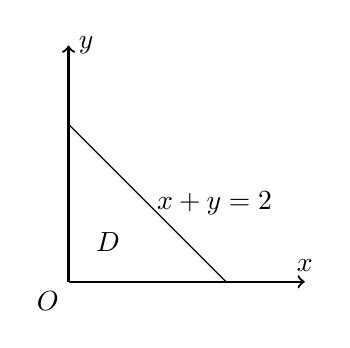
\begin{tikzpicture}
			\draw[thick,->] (0,0) -> (3,0)node[above]{\(x\)};
			\draw[thick,->] (0,0) -> (0,3)node[right]{\(y\)};
			\draw (.5,.5)node{\(D\)};
			\draw (0,0)node[below left]{\(O\)};
			\draw (0,2)--(2,0)node[midway,right]{\(x+y=2\)};
		\end{tikzpicture}
		\subcaption{}
	\end{subfigure}%
	\begin{subfigure}[b]{\subwidth}
		\centering
		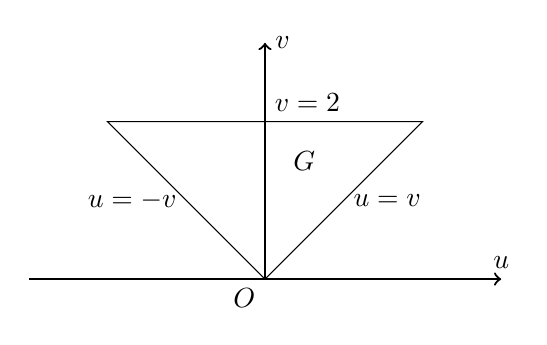
\begin{tikzpicture}
			\draw[thick,->] (-3,0) -> (3,0)node[above]{\(u\)};
			\draw[thick,->] (0,0) -> (0,3)node[right]{\(v\)};
			\draw (.5,1.5)node{\(G\)};
			\draw (0,0)node[below left]{\(O\)};
			\draw (0,0)--(2,2)node[midway,right]{\(u=v\)}
				--(-2,2)node[midway,above right]{\(v=2\)}
				--(0,0)node[midway,left]{\(u=-v\)};
		\end{tikzpicture}
		\subcaption{}
	\end{subfigure}%
	\caption{}
\end{figure}

雅克比式为\[
	J(u,v)
	= \jacobi{x,y}{u,v}
	= \def\arraystretch{1.5} \begin{vmatrix}
	-\frac12 & \frac12 \\
	\frac12 & \frac12
	\end{vmatrix}
	= - \frac12.
\]
那么\begin{align*}
	\iint_D \exp(\frac{y-x}{y+x}) \dd{x} \dd{y}
	&= \iint_G \exp(\frac{u}{v}) \abs{-\frac12} \dd{u} \dd{v} \\
	&= \frac12 \int_0^2 \dd{v} \int_{-v}^v \exp(\frac{u}{v}) \dd{u} \\
	&= \frac12 \int_0^2 \left( e - e^{-1} \right) v \dd{v}
	= e - e^{-1}.
\end{align*}
\end{solution}
\end{example}

\begin{example}
计算\(\iint_D \sqrt{1 - \frac{x^2}{a^2} - \frac{y^2}{b^2}} \dd{x} \dd{y}\),
其中\(D\)是椭圆\(\frac{x^2}{a^2} + \frac{y^2}{b^2} = 1\ (a,b>0)\)所围成的闭区域.
\begin{solution}
作广义极坐标变换\[
	\left\{ \begin{array}{l}
		x = a \rho \cos\theta, \\
		y = b \rho \sin\theta.
	\end{array} \right.
\]
在这变换下,与\(D\)对应的闭区域为
\(G = \Set{(\rho,\theta) \given 0\leq\rho\leq1,0\leq\theta\leq2\pi}\),
雅克比式\[
	J = \jacobi{x,y}{\rho,\theta} = ab\rho.
\]
由于\(J\)仅当\(\rho=0\)时为零,
所以换元公式仍成立,
从而有\[
	\iint_D \sqrt{1 - \frac{x^2}{a^2} - \frac{y^2}{b^2}} \dd{x} \dd{y}
	= \iint_G \sqrt{1-\rho^2} ab\rho \dd{\rho} \dd{\theta}
	= \frac23 \pi ab.
\]
\end{solution}
\end{example}
